\documentclass[runningheads]{llncs}
\usepackage{graphicx}
\usepackage{todonotes}
\usepackage{svg}
\usepackage{pgfplots}
\DeclareUnicodeCharacter{2212}{−}
\usepgfplotslibrary{groupplots,dateplot}
\usetikzlibrary{patterns,shapes.arrows}
\pgfplotsset{compat=newest}



\begin{document}

\title{Cloud Computing \& Big Data}
\author{Riley Evans - re17105}
\institute{University of Bristol}
\maketitle 


\begin{abstract}
The use of cloud computing for executing embarrassingly parallel tasks is now easier that ever. Tasks are able to scale many instances with ease, without the overhead of managing many machines. This report will implement an example of one of these tasks - a coursework submission auto marker.
\end{abstract}

\section{The Task \& Motivation}
The embarrassingly parallel task chosen for implementation is an auto-marker for students Game of Life coursework submissions. This involves ensuring that all the tests pass and running benchmarks on the solution so that markers can compare the efficiency of each submission. 

This task is suited to processing in an embarrassingly parallel fashion - each submission has the same process run on it. It is also beneficial to run this task in a scalable environment for several reasons. Firstly, each submission can take from a few minutes to mark up to 84 minutes in the worst-case scenario depending on if a student has deadlocks present in their code. With the ever-increasing demand for quicker feedback and increasing student numbers, it would be helpful if this task could be parallelised to speed up the marking of coursework. Secondly, if there is one slow submission it would not be ideal if it blocked the marking of every other submission. 

Another justification for running it on the cloud is that it provides multiple machines all of the same specification. One could argue that if each marker were to run separate batches of submissions on their own personal machines, it could lead to inconsistencies when marking. Especially, if each marker has a different specification machine. On a cloud provider, using the same instance tier results in identical machines being provisioned.

\section{The Architecture}

The architecture can be divided into two sections - client facing and submission processing. Fig. \ref{fig:client-interaction}, shows how a client interacts with the system and the components that are accessible to it. A client will initially invoke a Lambda function to register itself as a client in the system. The Lambda function will then return a client ID along with an SQS queue for it to listen for results on. The client then uploads zip files to an S3 bucket. Once a submission has been processed a message will be sent to the client's SQS queue. The client is then able to download the file from an S3 bucket. The client has two different modes: asynchronous or synchronous. The asynchronous mode is helpful when marking can take longer that the 3 hours than the AWS Educate access keys are active for. By assigning client IDs the system is capable of differentiating work between each client. This means that it is able to handle multiple clients at the same time.

\begin{figure}[ht]
\vspace{-1em}
    \centering
    \includegraphics[scale=0.38]{architecture-diagrams/client_interaction.png}
    \vspace{-2em}
    \caption{Client interaction diagram}
    \label{fig:client-interaction}
    \vspace{-1em}
\end{figure}

The submission processing part of the system is illustrated in Fig. \ref{fig:architecture}. This depicts how a submission is taken from one S3 bucket and converted into a report PDF in a second bucket. The architecture has 3 key components, the Elastic Container Service (ECS) cluster, the Simple Queuing System (SQS) and the Lambda functions used for auto-scaling. 

\begin{figure}[ht]
\vspace{-1em}
    \centering
    \includegraphics[scale=0.18]{architecture-diagrams/architecture-6.png}
    \vspace{-1em}
    \caption{System Architecture diagram}
    \label{fig:architecture}
    \vspace{-1em}
\end{figure}

The auto-mark script that is used to produce a report for the submission is run inside a docker container, there are several reasons why this is suitable. Firstly, it means that the marking of each submission can be contained, this prevents the student from running malicious code, that could either cause problems with the host machine or another students submission. Secondly, it allows a specification to be given to students so that they can ensure that their submission will run inside the environment without problems. This will help build confidence between students and markers.

Each container will run within the Elastic Container Service. In order to do this a task definition is needed, this states what container image will be run and any resource allocations that it requires. For example the auto-mark task requires 4096 CPU units, this is equivalent to 4 full CPU cores. A service is then specified within the cluster, this will be able to schedule tasks on available EC2 container instances. The service is able to control the number of desired tasks running. It ensures that the containers running on an EC2 instance do not exceed the maximum resources that it has available. If a container crashes or becomes unhealthy, the service will be able to stop that container and start a new one in its place.

The auto-mark SQS queue is used to manage a list of all the submissions that need marking. This helps to provide fault tolerance within the system - discussed later in the report. Uploads to the S3 upload bucket will trigger a message to be sent to the queue, and tasks within the ECS cluster will request messages from this queue so they know which zip files to mark.


\section{Auto Scaling}
There are many parts of the academic year where having this system running EC2 instances would be a waste of money, as there is no work to mark. However, towards the end of term there could be large demand from lecturers who would like to auto-mark work. Therefore, the ability for this system to auto-scale is crucial. Ideally, when this system is not being used it uses the least amount of resources possible to avoid costs being incurred.

Initially, one solution that presented itself was to use the auto-scaling built into ECS. However, after investigation, there were several problems with this approach. The auto-scaling system did not easily allow for control over which instance would be terminated, which could be problematic. If we are marking submissions on 7 out of the 8 running container instances with no more work to do, then ideally the one not marking would be terminated. However, this is difficult to do when not controlling which instance is terminated. Instead, an instance that is currently marking a submission could be terminated causing it to fail to mark a submission. 

Another solution to this problem could be to invoke a Lambda function on a schedule - similar to a cron job. This would be able to check the state of the queue and decide when to start more instances or which instances to terminate. However, this comes with the problem that a lambda will be invoked, even when there is no need to. Additionally, AWS Educate prevents recurring Lambdas.

The auto-scaling solution implemented aims to solve both of these problems. When work is added the the auto-mark queue then a Lambda function will be triggered to check if an instance needs to be started. The Lambda function is able to start at most 4 instances in a single invocation. This allows for the number of instances to rapidly grow when tasks are added to the queue. Instances are shutdown by reporting their status to another Lambda when they have not processed any work for a set period of time - 200 seconds. One could question what happens if a container is faulty and not able to report its state. In this scenario it will be reported as unhealthy and stopped. The effect of this auto scaling solution can be seen in Fig. \ref{fig:scale-graph}, this example uses a maximum of 8 instances.

\begin{figure}[ht]
    \vspace{-1em}
    \centering
    % This file was created by tikzplotlib v0.9.6.
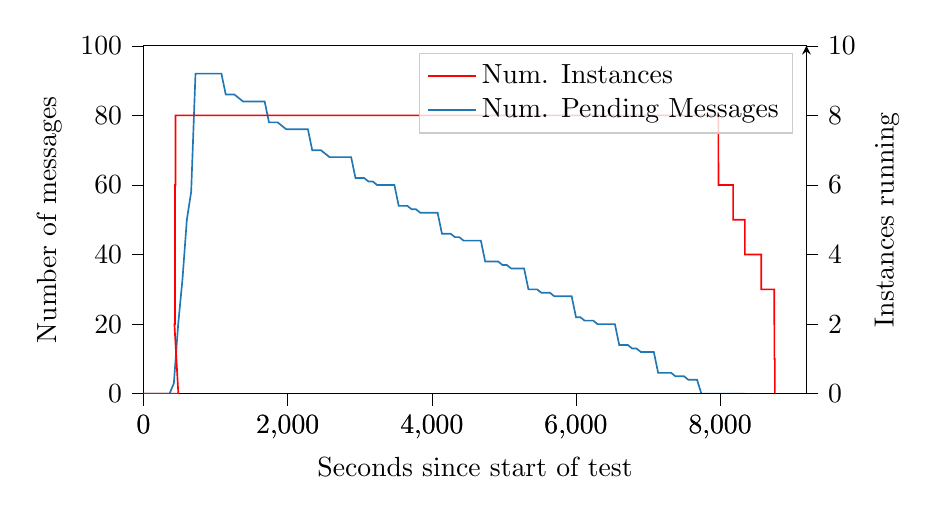
\begin{tikzpicture}

\definecolor{color0}{rgb}{0.12156862745098,0.466666666666667,0.705882352941177}

\begin{axis}[
height=6cm,
width=10cm,
tick align=outside,
tick pos=left,
x grid style={white!69.0196078431373!black},
xlabel={Seconds since start of test},
xmin=0, xmax=9198,
xtick style={color=black},
y grid style={white!69.0196078431373!black},
ylabel={Number of messages},
ymin=0, ymax=100,
ytick style={color=black}
]
\addplot [semithick, color0]
table {%
0 0
60 0
120 0
180 0
240 0
300 0
360 0
420 3
480 20
540 33
600 50
660 58
720 92
780 92
840 92
900 92
960 92
1020 92
1080 92
1140 86
1200 86
1260 86
1320 85
1380 84
1440 84
1500 84
1560 84
1620 84
1680 84
1740 78
1800 78
1860 78
1920 77
1980 76
2040 76
2100 76
2160 76
2220 76
2280 76
2340 70
2400 70
2460 70
2520 69
2580 68
2640 68
2700 68
2760 68
2820 68
2880 68
2940 62
3000 62
3060 62
3120 61
3180 61
3240 60
3300 60
3360 60
3420 60
3480 60
3540 54
3600 54
3660 54
3720 53
3780 53
3840 52
3900 52
3960 52
4020 52
4080 52
4140 46
4200 46
4260 46
4320 45
4380 45
4440 44
4500 44
4560 44
4620 44
4680 44
4740 38
4800 38
4860 38
4920 38
4980 37
5040 37
5100 36
5160 36
5220 36
5280 36
5340 30
5400 30
5460 30
5520 29
5580 29
5640 29
5700 28
5760 28
5820 28
5880 28
5940 28
6000 22
6060 22
6120 21
6180 21
6240 21
6300 20
6360 20
6420 20
6480 20
6540 20
6600 14
6660 14
6720 14
6780 13
6840 13
6900 12
6960 12
7020 12
7080 12
7140 6
7200 6
7260 6
7320 6
7380 5
7440 5
7500 5
7560 4
7620 4
7680 4
7740 0
7800 0
7860 0
7920 0
7980 0
8040 0
8100 0
8160 0
8220 0
8280 0
8340 0
};

\end{axis}

\begin{axis}[
height=6cm,
width=10cm,
axis y line=right,
legend cell align={left},
legend style={fill opacity=0.8, draw opacity=1, text opacity=1, draw=white!80!black},
tick align=outside,
x grid style={white!69.0196078431373!black},
xmin=0, xmax=9198,
xtick pos=left,
xtick style={color=black},
y grid style={white!69.0196078431373!black},
ylabel={Instances running},
ymin=0, ymax=10,
ytick pos=right,
ytick style={color=black}
]
\addplot [semithick, red]
table {%
0 0
482 0
428 2
435 2
435 6
443 6
443 8
7976 8
7976 7 
7977 6
8180 6
8180 5
8344 5
8344 4
8570 4
8570 3
8752 3
8752 2
8753 2
8753 1
8760 1
8760 0
};
\addlegendentry{Num. Instances}

% Just to make it go on legend...
\addplot [semithick, color0]
table {%
0 0
};
\addlegendentry{Num. Pending Messages}
\end{axis}

\end{tikzpicture}

    \caption{How the number of active instances scales with the number of pending messages.}
    \label{fig:scale-graph}
    \vspace{-1em}
\end{figure}

One benefit of this system is that when no jobs running you can have no instances running. This will reduce the standby cost of the system, especially since Lambda functions are only charged when they are run - the standby cost of this system is \$0.00.


% Use auto-scaling group and scale-in protection? Will fix unhealthy ec2 instances automatically. And keep the desired number up.

\section{System Performance}
Being able to process submissions quickly would be an ideal feature of this system. The system runtime, however, will be limited by the length of time each submission takes to mark - this can vary significantly. Using an average timed solution, the throughput of the system can be calculated. To do this the time will be measured for 100 submissions to be processed, from the first upload time to the last download time. The system executed for a total of 133 minutes and completed 100 submissions giving a throughput of 0.75 submissions per minute. 

The system startup time can be estimated from the latency it takes to complete the first submission. In this case the latency was 12 minutes. With each submission taking between 10-11 minutes, this would suggest that our system has a startup time of roughly 1-2 minutes. A breakdown of where time is spent can be seen in Table \ref{table:startup-time}. Each task in the startup process is dependent on the previous, therefore giving a startup time of 81 seconds. 

\begin{table}
\vspace{-1em}
\caption{Startup time of each component in the system}\label{tab1}
\centering
\begin{tabular}{|c|c|}
\hline
\textbf{Task} & \textbf{Runtime (s)} \\
\hline
Auto-Mark Lambda & 1 \\
Scale Up Lambda & 6 \\
EC2 Instance Start & 43 \\
ECS Image Pulling & 31 \\
\hline
\textbf{Total} & 81 \\
\hline
\end{tabular}
\label{table:startup-time}
\vspace{-1em}
\end{table}

It is also worth comparing this cloud based solution to another possible way of marking the submissions. They could be marked on a single machine in a sequential fashion. It would not be possible to run them in parallel as the submissions need full access to \emph{all} CPU cores. A single submission took 10 minutes 42 seconds to run on a 4-core i5-4690 processor. From this It can be estimated that 100 submissions would 17 hours 15 minutes. This is significantly slower than the 2 hours 13 minutes for the cloud based solution. This would mean that a lecturer spends more time waiting for the submissions to be marked, and would therefore have less time to give more detailed feedback.

\section{Cost}
To evaluate the cost of the system, a sample of 100 submissions can be run on the system, and then evaluating the number of resources used. The breakdown of the costs can be seen in Table \ref{table:costing}. To estimate the cost of the EC2 instances, the length of time they ran for needs to be calculated. This can be calculated from the area under the curve of the number of instances shown in Fig. \ref{fig:scale-graph}. This results in a value of 63830 seconds of running instances - EC2 instances are charged per second~\cite{ec2-per-second}. The EC2 instances are the most major cost in this system - they represent 98.3\% of the total costs. The instance type chosen was c4.xlarge, this is because that type was recommended to the students to use. Therefore, it would not be possible to use a different one to reduce the costs.

The usage of Lambda, SQS and S3 are all included in the free-tier, however, the costs excluding the free-tier are also calculated. They are small enough to end up with a cost of \$0.00. Lambda invocations are charged at \$0.0000166667 for every GB of RAM used per second. The average runtime of each Lambda function is estimated to be 3 seconds and all Lambdas use just 128MB of RAM. S3 is billed at \$$3.2\times10^{-5}$ per GB-hour, with each submission using on average 4.1MB this can be estimated to 0.4GB. The number of hours is rounded up to 3 hours as any usage within a one hour period will get rounded up, for example 2 hour 20 minutes of usage will be billed at 3 hours.

\begin{table}
\vspace{-1em}
\caption{Costs of the system}
\centering
\begin{tabular}{|c||c|c|c|}
\hline
\textbf{Resource} & \textbf{Usage} & \textbf{Cost per unit (\$)} & \textbf{Cost} \\
\hline
EC2 (c4.xlarge) & 63830s & 0.00005528 & \$3.53 \\
EBS (general purpose) & 63830s $\times$ 30GB & $3\times10^{-8}$ & \$0.06 \\
Lambda Invocations & 208 $\times$ 3s $\times$ 0.125GB & 0.0000166667 & \$0.00 \\
SQS & 200 & $4\times10^{-7}$ & \$0.00 \\
S3 (general storage) & 3hr $\times$ 0.4GB & $3.2\times10^{-5}$ & \$0.00 \\
\hline
\multicolumn{3}{|r|}{\textbf{Total}} & \$3.59 \\
\hline
\end{tabular}
\label{table:costing}
\vspace{-1em}
\end{table}

A key comparison for the cost could be comparing it to the costs of running in on a local machine. Previously it was calculated that running on a single machine would take 17 hours 15 minutes. Assuming the machine draws 450W of power, this converts to 8 kWh. The cost of power can be calculated as $8 \times 0.163\cite{avg-kwh-cost} = \pounds1.304 \approx \$1.74$. The cost of ownership has not been factored in here, as the machine will already be owned by the marker. This cost is lower than the cost of running the system on AWS, however, it does lockup a machine for 16 hours that cannot be used to avoid interfering with the benchmark times - which could have downsides if other work needs completing at the same time.


\section{Fault Injection}
Fault tolerance is crucial when marking the submissions: it would not be good if a student has a viva and their submission had failed to process. This system is capable of resolving faults that may occur. 

There are several ways this system could fail, firstly, the Python script that is marking could fail. If this occurs then the container stops running and a new one will be started on the container instance. However, the submission that it was processing will have already been taken out of the SQS queue. In order to be fault tolerant this submission will need to be re-added to the queue, this is possible through an SQS feature - the visibility timeout. When a message is received from the queue, a timeout is set, if this timeout expires before the recipient has deleted the message then it will be re-added to the queue automatically. Each submission could take from 5 minutes up to 84 minutes to mark depending on how good the submission is. Therefore, it would make sense to set the higher as the timeout, however, if one submission fails it could extend the total processing time significantly. It is possible to extend the visibility timeout multiple times after receiving the message. This could be used to allow the timeout to be updated regularly, preventing a large delay from the task failing to when it is decided that it failed. Using this incremental timeout between each subset of tests, the failure reporting delay can be reduced to at most 36 minutes and as little as 30 seconds - a reduction of between 57\% and 99\%.

This can be tested by adding random crashes to the python script, and observing its effects on the throughput of the system. Between each set of testing a failure can be added at a rate of 1\% - giving each task a probability of failure of 8\%. As previously done, 100 test submissions can be run through the system, the results of which can be seen in Fig. \ref{fig:faulty-system-hidden} \& Fig. \ref{fig:faulty-system-visible}. 


\begin{figure}
\vspace{-1em}
\centering
\begin{minipage}{.475\textwidth}
  \centering
  % This file was created by tikzplotlib v0.9.6.
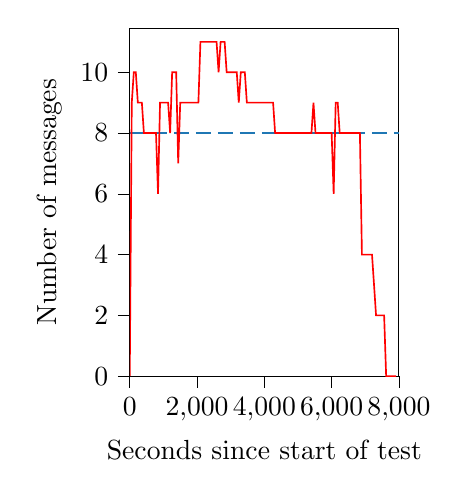
\begin{tikzpicture}

\definecolor{color0}{rgb}{0.12156862745098,0.466666666666667,0.705882352941177}

\begin{axis}[
height=6cm,
width=5cm,
tick align=outside,
tick pos=left,
x grid style={white!69.0196078431373!black},
xlabel={Seconds since start of test},
xmin=0, xmax=8000,
xtick style={color=black},
y grid style={white!69.0196078431373!black},
ylabel={Number of messages},
ymin=0, ymax=11.45,
ytick style={color=black},
ytick={0, 2, 4, 6, 8, 10}
]
\path [draw=color0, semithick, dash pattern=on 5.55pt off 2.4pt]
(axis cs:0,8)
--(axis cs:8000,8);

\addplot [semithick, red]
table {%
0 0
60 9
120 10
180 10
240 9
300 9
360 9
420 8
480 8
540 8
600 8
660 8
720 8
780 8
840 6
900 9
960 9
1020 9
1080 9
1140 9
1200 8
1260 10
1320 10
1380 10
1440 7
1500 9
1560 9
1620 9
1680 9
1740 9
1800 9
1860 9
1920 9
1980 9
2040 9
2100 11
2160 11
2220 11
2280 11
2340 11
2400 11
2460 11
2520 11
2580 11
2640 10
2700 11
2760 11
2820 11
2880 10
2940 10
3000 10
3060 10
3120 10
3180 10
3240 9
3300 10
3360 10
3420 10
3480 9
3540 9
3600 9
3660 9
3720 9
3780 9
3840 9
3900 9
3960 9
4020 9
4080 9
4140 9
4200 9
4260 9
4320 8
4380 8
4440 8
4500 8
4560 8
4620 8
4680 8
4740 8
4800 8
4860 8
4920 8
4980 8
5040 8
5100 8
5160 8
5220 8
5280 8
5340 8
5400 8
5460 9
5520 8
5580 8
5640 8
5700 8
5760 8
5820 8
5880 8
5940 8
6000 8
6060 6
6120 9
6180 9
6240 8
6300 8
6360 8
6420 8
6480 8
6540 8
6600 8
6660 8
6720 8
6780 8
6840 8
6900 4
6960 4
7020 4
7080 4
7140 4
7200 4
7260 3
7320 2
7380 2
7440 2
7500 2
7560 2
7620 0
7680 0
7740 0
7800 0
7860 0
7920 0
};
\end{axis}

\end{tikzpicture}

    \caption{The number of hidden messages.}
    \label{fig:faulty-system-hidden}
\end{minipage}%
\hspace{0.045\textwidth}%
\begin{minipage}{.475\textwidth}
  \centering
  % This file was created by tikzplotlib v0.9.6.
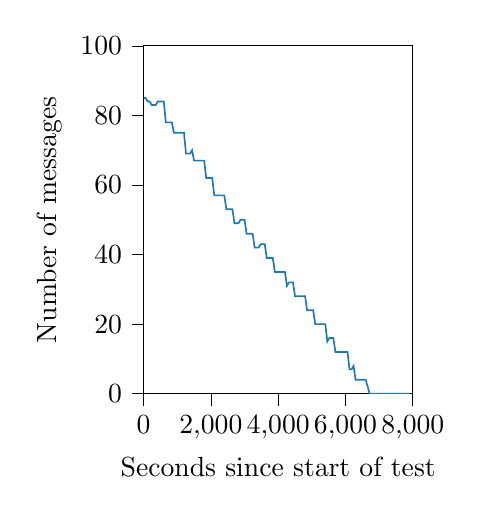
\begin{tikzpicture}

\definecolor{color0}{rgb}{0.12156862745098,0.466666666666667,0.705882352941177}

\begin{axis}[
height=6cm,
width=5cm,
tick align=outside,
tick pos=left,
x grid style={white!69.0196078431373!black},
xlabel={Seconds since start of test},
xmin=0, xmax=8000,
xtick style={color=black},
y grid style={white!69.0196078431373!black},
ylabel={Number of messages},
ymin=0, ymax=100,
ytick style={color=black}
]
\addplot [semithick, color0]
table {%
0 85
60 85
120 84
180 84
240 83
300 83
360 83
420 84
480 84
540 84
600 84
660 78
720 78
780 78
840 78
900 75
960 75
1020 75
1080 75
1140 75
1200 75
1260 69
1320 69
1380 69
1440 70
1500 67
1560 67
1620 67
1680 67
1740 67
1800 67
1860 62
1920 62
1980 62
2040 62
2100 57
2160 57
2220 57
2280 57
2340 57
2400 57
2460 53
2520 53
2580 53
2640 53
2700 49
2760 49
2820 49
2880 50
2940 50
3000 50
3060 46
3120 46
3180 46
3240 46
3300 42
3360 42
3420 42
3480 43
3540 43
3600 43
3660 39
3720 39
3780 39
3840 39
3900 35
3960 35
4020 35
4080 35
4140 35
4200 35
4260 31
4320 32
4380 32
4440 32
4500 28
4560 28
4620 28
4680 28
4740 28
4800 28
4860 24
4920 24
4980 24
5040 24
5100 20
5160 20
5220 20
5280 20
5340 20
5400 20
5460 15
5520 16
5580 16
5640 16
5700 12
5760 12
5820 12
5880 12
5940 12
6000 12
6060 12
6120 7
6180 7
6240 8
6300 4
6360 4
6420 4
6480 4
6540 4
6600 4
6660 2
6720 0
6780 0
6840 0
6900 0
6960 0
7020 0
7080 0
7140 0
7200 0
7260 0
7320 0
7380 0
7440 0
7500 0
7560 0
7620 0
7680 0
7740 0
7800 0
7860 0
7920 0
};
\end{axis}

\end{tikzpicture}

    \caption{The number of visible messages.}
    \label{fig:faulty-system-visible}
\end{minipage}
\vspace{-1em}
\end{figure}


% \todo[inline]{blah blah about what graph shows}
Fig. \ref{fig:faulty-system-hidden}, visualises the number of hidden messages in the queue. The hidden messages will include all messages that have been accepted out of the queue, but not marked as complete. In this example - where 8 marker tasks are being run in parallel - any value in this graph above 8 shows that there has been a failed task. This is useful for monitoring the system to view how many failed tasks have occurred. At the 2000 second mark, there were 3 task that had all failed but their timeout had not been exceeded yet. Over the next 2000 seconds it can be visualised when the timeouts trigger and the task is moved from hidden to visible again. Fig. \ref{fig:faulty-system-visible}, demonstrates the number of visible messages in the queue at any point in the marking process. You can align any uptick in the number visible messages to points in Fig. \ref{fig:faulty-system-hidden} where the number of hidden tasks decrease back down towards 8. This trend does not apply past 6500 seconds.

The auto-marker container also has a health check to ensure that stays healthy. In a similar method to the queue timeout, a status update is output to a file. This file can be checked to decide if the container is still healthy or if there is a problem. For example, the Game of Life makes use of parallel workers, this could result in deadlocks. Although timeouts have been used, there is the possibility that the Python script could get stuck waiting for a submission that has deadlocked. In this case the health check would fail as the script would not report a new status in the correct period of time. If the health check fails multiple times the container will be stopped and a new one started to replace it. 


\section{Conclusion \& Future Work}
In this report, a system has been presented that allows for the auto marking of students coursework submissions in the cloud. It has been demonstrated how the system is able to successfully scale based on demand in the queue, and how when there is no demand the system costs \$0.00 to keep in standby. Finally, presenting method for ensuring that the system remains fault tolerant, that ensures that all work is processed with the minimal delay when certain tasks fail.

There are, however, some possible improvements that could be made to make the system even more capable. Firstly, an adversary could take advantage of a client to interfere with processing as they have full access to the AWS API. It would be more secure if a client could be granted access tokens that only allowed access to the certain areas that they need. They could then use a public REST API to invoke the Lambda function, which would return their credentials. Unfortunately due to the restrictions on AWS Educate this was not possible, but if this system was used more widely in the future this would be critical. 

Secondly, in its current state the system only supports marking of Game of Life courseworks. A future expansion could allow for the marking of different types of coursework, for example, marking C code submissions. It can be hypothesised that when a client is created, they are able to also specify a container of their own construction. This would then have 2 attached volumes: a submission volume and an artefacts volume. The container could then store the results of auto-marking in the artefacts volume, which would be forwarded to the client. This would allow the system to be more widely used.  


\begin{thebibliography}{8}

\bibitem{ec2-per-second} AWS News Blog. Per-Second Billing for EC2 Instances and EBS Volumes. \url{https://aws.amazon.com/blogs/aws/new-per-second-billing-for-ec2-instances-and-ebs-volumes/}

\bibitem{avg-kwh-cost} Department for Business, Energy \& Industrial Strategy. Annual domestic energy bills. https://www.gov.uk/government/statistical-data-sets/annual-domestic-energy-price-statistics

\end{thebibliography}

\section*{Appendix}
\subsection*{How to deploy \& run the system}

The source code for this implementation can be found in the GitHub repository \url{https://github.com/ccdb-uob/CW20-06}. The version used to measure the fault tolerance can be found on the branch \texttt{faulty-version} at \url{https://github.com/ccdb-uob/CW20-06/tree/faulty-version}.

The deployment instructions can be found in the \texttt{README.md} of the repository (\url{https://github.com/ccdb-uob/CW20-06/blob/main/README.md}). 

\end{document}
